\documentclass[../main.tex]{subfiles}
\begin{document}
\chapter{Achievability of the Channel Coding Theorem}
To prove achievability:\begin{itemize}
    \item Consider a DMC (discrete memoryless channel)  $p(y|x)$.
    \item For every input distribution $p(x)$, prove that the rate $I(X;Y)$ is achievable by showing for large $n$ the existence of a channel code such that \begin{itemize}
        \item the rate of the code is arbitrarily close to $I(X;Y)$
        \item the maximal probability of error $\lambda_max$ is arbitrarily small.
    \end{itemize}
    \item Choose the input distribution $p(x)$ to be the one that achieves the channel capacity, i.e. $I(X;Y)=c$
\end{itemize}
\begin{bbox}{Lemma: upper bound of the probability of generation being jointly typical}
    Let $(\vec X', \vec Y')$ be $n$ iid copies of a pair of generic random variables $(X', Y')$ and $X'$ and $Y'$ are independent. Then \[
    \Pr\{(\vec X',\vec Y')\in T^n_{XY_\delta}\} \leq 2^{-n(I(X;Y)-\tau)}
    \] where $\tau\to 0$ as $\delta \to 0.$
    \begin{proof}
        Consider \[
        Pr((\vec X', \vec Y')\in T^n_{XY_\delta} )= \sum_{\vec x, \vec y\in T}p(\vec x) p(\vec y).
        \]
    By consistentcy of strong typicality, for each $(\vec x, \vec y) \in T_{XY}$, $\vec x$ and $\vec y$ are both marginally typical.
    \newline
    By the strong AEP, 
    \[
    p(\vec x)\leq 2^{-n(H(X)-\eta)}
    \] and \[
    p(\vec y) \leq 2^{-n(H(Y)-\zeta)}
    \]
    where $\eta, \zeta\to 0$ as $\delta \to 0$.
    \newline
    By the strong JAEP, \[
    |T^n_{XY_\delta}|\leq 2^{n(H(X,Y)+\xi)}
    \] where $\xi\to 0$ as $\delta \to 0$.
Then \begin{align*}
    &\Pr\{(\vec X', \vec Y')\in T^n_{XY_\delta}\}\\
    &=\sum_{(\vec x, \vec y)\in T}p(\vec x)p(\vec y)\\
    &\leq 2^{n(H(X,Y)+\xi)}\times 2^{-n(H(X)-\eta)}\times 2^{-n(H(Y)-\zeta)}\\
    &=2^{-n(I(X;Y)-\tau)}
\end{align*}
where $\tau = \zeta + \eta + \zeta\to 0$ as $\delta \to 0$
    \end{proof}
\end{bbox}
This lemma seems counter-intuitive because the probability of a generated sequence being jointly typical is supposed to be large, but this makes sense because: we generate the sequence $X'$ iid wrt the distribution $p(x)$ and generate the other sequence $Y'$ iid wrt $p(y)$. The 2 generation processes are independent. However, $X$ and $Y$ are not necessarily independent. The less independent they are, the less likely that $(\vec X', \vec Y')$ generated in this fasion is typical.
\begin{pbox}{Interpretation of the above lemma}
    Consider the quasi-uniform array where the rows are typical $x$ sequences and the columns are typical $y$ sequences.
    \begin{itemize}
        \item Randomly choose a row with uniform distribution and randomly choose a column with uniform distribution.
        \item Then \[
        \Pr\{\text{obtaining a jointly typical pair}\} \approx \frac{2^{nH(X,Y)}}{2^{nH(X)}2^{nH(Y)}} = 2^{-nI(X;Y)}
        \]
    \end{itemize}
\end{pbox}
\centering{Random Coding Scheme}
Parameter settings \begin{itemize}
    \item Fix $\epsilon>0$ and input distribution $p(x)$. Let $\delta$ be specified later.
    \item Let $M$ be an even integer such that \[
    I(X;Y)-\frac{\epsilon}{2}<\frac{1}{n}\log M = \text{rate of the code} < I(X;Y)-\frac{\epsilon}{4}
    \] where $n$ is sufficiently large, i.e. $M\approx 2^{nI(X;Y)}$
    \item The lower bound guarantees that the rate is close to $I(X;Y)$. The upper bound guarantees that the rate is not too close to $I(X;Y)$.
\end{itemize}
The Random Coding Scheme:
\begin{itemize}
    \item 1. Construct the codebook $\mathcal{C}$ of an $(n,M)$ code by generating $M$ codewords in $\X^n$ independently and identically accoding to $p(x)^n$. Denote these codewords by $\vec X(1),\vec X(2), \dots, \vec X(M)$
    \item Generate each component accoding to $p(x)$
    \item There are a total of $|\X|^{Mn}$ possible codebooks that can be constructed.
    \item Regard two codebooks whose sets of codewords are permutations of each other as two different codebooks.
    \item 2. Reveal the codebook $\mathcal{C}$ to both the encoder and the decoder.
    \item 3. A message $W$ is chosen from $\mathcal{W}$ according to the uniform distribution.
    \item 4. Transmit $\vec X=\vec X(W)$ through the channel.
    \item The channel outputs a sequence $Y$ according to \[
    \Pr(\vec Y=\vec y|\vec X(W)=\vec x) = \prod_{i=1}^np(y_i|x_i).
    \] 
    \item 6. The sequence $\vec Y$ is decoded to the message $w$ if $(\vec X(w), \vec Y)\in T^n_{XY_\delta}$ and there does not exists $w'\neq w$ such that $(\vec X(w'), \vec Y)\in T^n_{XY_\delta}$. Otherwise, $\vec Y$ is decoded to some constant message in $\mathcal{W}$. Denote the message to which $\vec Y$ is decoded to by $\hat{W}.$
\end{itemize}
\section{Performance Analysis}
\begin{itemize}
    \item We need to show that $\Pr\{Error\}=\Pr\{\hat{W}\neq W\}$ can be made arbitrarily small.
    \item Consider \[
    \Pr\{Error\} = \sum_{w=1}^M \Pr\{Error|W=w\}p(W=w)
    \]\[
    \]
    This is equal to \[
    \Pr\{Error|W=1\}\sum_{w=1}^M\Pr\{W=w\} = \Pr\{Error|W=1\}
    \] by the construction of the Random Coding Scheme. All codewords are generated randomly in the same fashion.
    \item Assume without loss of generality that message $1$ is chosen.
    \item For $1\leq w\leq M$, define the event \[
    E_w := \{(\vec X(w), \vec Y)\in T^n_{XY_\delta}\}
    \]
    \item If $E_1$ occurs but $E_w$ does not occur for all $2\leq w\leq M$, then no decoding error, because according to our decoding rule, the decoded message $\hat{W}$ will be $1$. Therefore \[
    \Pr\{Error^C|W=1\} \geq \Pr\{E_1\cap E_2^C\cap \dots\cap E_M^C|M=1\}
    \]
    \item Consider \[
    \Pr\{Err|W=1\} = 1-\Pr\{Err^C|W=1\}
    \]
    \[
    \leq 1- \Pr\{E_1\cap E_2^C\cap \dots\cap E_M^C|W=1\}
    \]
    \[
    = \Pr\{E_1^C\cup E_2\cup \dots\cup E_M|W=1\}
    \]
    \item By the union bound, \[
    \Pr\{Err|W=1\}\leq \Pr\{E_1^C|W=1\}+\sum_{w=2}^M\Pr\{E_w|W=1\}
    \]
    \item By strong JAEP,
    \[
    \Pr\{E_1^C|W=1\}=\Pr\{(\vec X(1), \vec Y)\notin T^n_{XY_\delta}|W=1\}<\nu
    \]
    where $\nu \to 0$ as $\delta \to 0$
    \item Conditioning on $\{W=1\},$ for $2\leq w\leq M$, $(\vec X(w),\vec Y)$ are $n$ iid copies of the pair of generic random variables $(X',Y')$ where $X'\sim X$ and $Y'\sim Y$.
    \item Since DMC is memoryless, $X'$ and $Y'$ are independent because $\vec X(1)$ and $\vec X(w)$ are independent and the generation of $\vec Y$ depends only on $\vec X(1)$.
    \item For $2\leq w\leq M$, \[
    \Pr\{E_w|W=1\}= \Pr\{(\vec X(w),Y)\in T^n_{XY_\delta}|W=1\}
    \]
    \[
    \leq 2^{-n(I(X;Y)-\tau)}
    \] where $\tau \to 0$ as $\delta \to 0.$
    \item Note that \[
    \frac{1}{n}\log M < I(X;Y)-\frac{\epsilon}{4}\iff M < 2^{n(I(X;Y)-\frac{\epsilon}{4}}
    \]
    \item Therefore, \[
    \Pr\{Err\} < \nu + 2^{n(I(X;Y)-\frac{\epsilon}{4})}\cdot 2^{-n(I(X;Y)-\tau)}
    \]
    \[
    =\nu + 2^{-n(\frac{\epsilon}{4}-\tau)}
    \]
    \item $\epsilon$ is fixed. Since $\tau\to 0$ as $\delta \to 0$, we can choose $\delta$ to be sufficiently small so that \[
    \frac{\epsilon}{4}-\tau > 0
    \]
    \item Then \[
    2^{-n(\frac{\epsilon}{4}-\tau)}\to 0
    \] as $n\to \infty$
    \item Let $\nu < \frac{\epsilon}{3}$, we get that \[
    Pr(Err) < \frac{\epsilon}{2}
    \] for sufficiently large $n$.
\end{itemize}
\centering{\textbf{Idea of Performance Analysis}}
\begin{itemize}
    \item Let $n$ be large.
    \item $\Pr(\vec X(1) \text{jointly typical with} \vec Y) \to 1$.
    \item For $w\neq 1$, $\Pr\{\text{$\vec X(w)$ jointly typical with $\vec Y$}\} \approx 2^{-nI(X;Y)}$.
    \item If $|\mathcal{C}|=M$ grows at a rate $<I(X;Y)$, then \[
    \Pr\{\text{$\vec X(w)$ jointly typical with $\vec Y$ for some $w\neq 1$}\} 
    \] can be made arbitrarily small.
    \item Then $\Pr\{\hat{W}\neq W\}$ can be made arbitrarily small.
\end{itemize}
\centering{\textbf{Existence of Deterministic Code}}
\begin{itemize}
    \item According to the random coding scheme, \[
    \Pr\{Err\}=\sum_C \Pr(C)\Pr\{Err|C\}
    \]
    \item Then there exists at least one codebook $C^*$ such that \[
    P_e=\Pr\{Err|C^*\}\leq \Pr\{Err\} < \frac{\epsilon}{2}
    \]
    \item By construction, this codebook has rate \[
    \frac{1}{n}\log M > I(X;Y)-\frac{\epsilon}{2}
    \], which can be arranged to be arbitrarily close to the channel capacity.
\end{itemize}
\centering{\textbf{Code with $\lambda_{max}<\epsilon$}}
\begin{itemize}
    \item We want a code with $\lambda_{max}<\epsilon$, not just $P-e<\frac{\epsilon}{2}$.
    \item Without loss of generality, assume $\lambda_1\leq \lambda_2\leq \dots\leq \lambda_M$. (ascending order) Consider \[
    \frac{1}{M}\sum_{w=1}^M\lambda_w < \frac{\epsilon}{2} iff \sum_{w=1}^M\lambda_w < \frac{M}{2}\epsilon
    \]
    Since $M$ is even, $M/2$
 is an integer. Then \[
 \sum_{w=M/2+1}^M\lambda_w < (\frac{M}{2})\epsilon\iff \frac{1}{M/2}\sum_{M/2+1}^M\lambda_w < \epsilon
 \]
 \item Conclusion: If $P_e<\frac{\epsilon}{2}$, then $\lambda_1\leq \lambda_2\leq \dots\leq \lambda_{M/2}<\epsilon$
 \item By discarding the worst half of the codewords in $C^*$, we have that $\lambda_{max}<\epsilon$.
 \item Then, the rate of the code becomes \[
 \frac{1}{n}\log \frac{M}{2} = \frac{1}{n}\log M-\frac{1}{n} > (I(X;Y)-\frac{\epsilon}{2})-\frac{1}{n} > I(X;Y)-\epsilon
 \] for sufficiently large $n$.
 \end{itemize}

 \section{Implication of the Channel Coding Theorem}
 The channel coding theorem says that an indefinitely long message can be communicated reliably through the channel when the block length $n\to \infty$. This is stronger than the requirement that the Bit Error Rate tending to $0$, because for long block length, even though BER can be small, the error rate of the whole message can be very large.
 \begin{itemize}
     \item The direct part of the channel coding theorem is an existential proof as opposed to a constructive proof.
     \item A randomly constructed code has the following issues: encoding and decoding are computationally prohibitive; high storage requirements for encoder and decoder.
     \item Nevertheless, the direct part implies that when $n$ is large, if the codewords are chosen randonly, most likely the code is good.
     \item The repetition code is not a good code because the numbers of $0$ and $1$ in the codewords are not roughly the same.
 \end{itemize}
 \begin{pbox}{Illustration of good code}
     \begin{itemize}
         \item We have approximately $2^{nI(X;Y)}$ codewords in $T^n_{X_\delta}$ 
         \item There are approximately $2^{nH(Y)}$ sequences in $T^n_{Y_\delta}$. 
         \item For each codeword that we choose from the x-typical set, it is jointly typical with approximately $2^{nH(Y|X)}$ y sequences 
         \item This set of $y$ sequences is represented by a cone. We want to pack as many codewords as possible such that these cones do not overlap.
         \item Therefore, the number of codewords cannot exceed about \[
         \frac{2^{nH(Y)}}{2^{nH(Y|X)}}=2^{nI(X;Y)}=2^{nC}
         \]
     \end{itemize}
 \end{pbox}
 Construction of codes with efficient encoding and decoding algorithms falls in the domain of channel coding theory. Performance of a code is measured by how far the rate is away from the channel capacity. All channel codes used in practice are linear in terms of computation and storage. Channel coding is widely used in all communications.

 
 \section{Feedback}
Feedback is common in practical communication systems for \textbf{correcting} possible errors which occur during transmission. Daily examples include phone call, classroom teaching. 
\newline
For data communication, the receiver may request a packey to be retransmitted if the parity check bits received are incorrect (Automatic Repeat-reQuest). The transmitter can decide what to transmit next based on the feedback on far.
\begin{itemize}
    \item Question: Can feedback increase the channel capacity?
    \item Not for DMC, even with complete feedback.
\end{itemize}
\begin{gbox}{Feedback Code}
    An $(n,M)$ code with \textbf{complete feedback} for a discrete memoryless channel with input alphabet $\X$ and output alphabet $\Y$ is defined by encoding functions \[
    f_i:\{1,2,\dots,M\}\times \Y^{i-1}\to \X
    \]
    for $1\leq i\leq n$ and a decoding function \[
    g:\Y^n \to \{1,2,\dots, M\}.
    \]
\begin{itemize}
    \item Notation: $\vec Y^{i}=(Y_1,Y_2,\dots, Y_i)$, $X_i=f_i(W,\vec Y^{i-1})$
    \item As we encode, we take information about the packets received by the receiver.
\end{itemize}
\end{gbox}
Dependency graph:
\[
q(w,\vec x,\vec y,\hat{w}) = q(w)(\prod_{i=1}^n q(x_i|w,\vec y^{i-1}))(\prod_{i=1}^np(y_i|x_i))q(\hat{w}|\vec y)
\]
\begin{gbox}{Achievable Rate with complete feedback}
    A rate $R$ is achievable with complete feedback for a discrete memoryless channel $p(y|x)$ if for any $\epsilon > 0$, there exists for sufficiently large $n$ and $(n,M)$ code with complete feedback such that \[
    \frac{1}{n}\log M > R-\epsilon
    \] and \[
    \lambda_{max} < \epsilon.
    \]
\end{gbox}
\begin{gbox}{Feedback Capacity}
The feedback capacity $C_{FB}$ of a discrete memoryless channel is the supremum over all the rates achievable by codes with complete feedback.
\newline
Note that a channel code without feedback is a speicial case of a channel code with complete feedback, so $C_{FB}\geq C$.
\end{gbox}
 \begin{bbox}{Lemma: Markov property of channel with feedback}
 For all $1\leq i\leq n$, \[
 (W,\vec Y^{i-1})\to X_i\to Y_i
 \] forms a Markov chain.
 \begin{proof}
     The Markov chain \[
     (W,\vec X^{i-1}, \vec Y^{i-1})\to X_i\to Y_i
     \] holds because the channel is memoryless. 
     \newline
     Then \[
     0 = I(W,\vec X^{i-1}, \vec Y^{i-1};Y_i,X_i)
     \]
     \[
     = I(W,\vec Y^{i-1};Y_i|X_i) + I(\vec X^{i-1}; Y_i|W,X_i,\vec Y^{i-1})
     \]
     By non-negative of Shannon's information measure, $I(W,\vec Y^{i-1};Y_i|X_i) = 0$, proving the Markov property.
 \end{proof}
 \end{bbox}
 
 \begin{bbox}{$C_{FB}\leq C$ for DMC}
    Consider any code with complete feedback.
    \newline
    Consider \[
    \log M = H(W) = I(W;\vec Y) + H(W|\vec Y)
    \]
    \begin{align*}
        I(W;\vec Y) &= H(\vec Y) - H(\vec Y|W)\\
        &= H(\vec Y) - \sum_{i=1}^n H(Y_i|\vec Y^{i-1}, W) \quad \text{by the chain rule}\\
        &= H(\vec Y) - \sum_{i=1}^n H(Y_i|\vec Y^{i-1},W,X_i), \quad \text{$X_i$ does not provide new information}\\
        &= H(\vec Y)-\sum_{i=1}H(Y_i|X_i) \quad \text{by Markov property}\\
        &\leq \sum_{i=1}^nH(Y_i)- \sum_{i=1}H(Y_i|X_i) \quad \text{by independence bound}\\
        &= \sum_{i=1}^n I(X_i;Y_i)\\
        &\leq nC
    \end{align*}
    \begin{align*}
        H(W|\vec Y)&=H(W|\vec Y, \hat{W}) \quad \text{since $\hat{W}$ is a function of $\vec Y$}\\
        &\leq H(W|\hat{W})\approx 0
    \end{align*}
    Then \[
    \log M \leq nC
    \]
    Rigorously, we can apply Fano's inequality to upper bound $H(W|\hat{W})$.
    \newline
    Lastly, we conclude that $R\leq C$ for any rate $R$ achievable with complete feedback.
 \end{bbox}
 Even though feedback does not increase the capacity of a DMC, the availability of feedback can make coding simpler.
 \newline
 Also if the channel has memory, feedback can increase the capacity.

 \section{Separation of Source and Channel Coding}
 \begin{itemize}
     \item Consider transmitting an information source with entropy rate $H$ reliably through a DMC with capacity $C$.
    \item If $H < C$, this can be achieved by separating source and channel coding without using feedback.
    \newline
    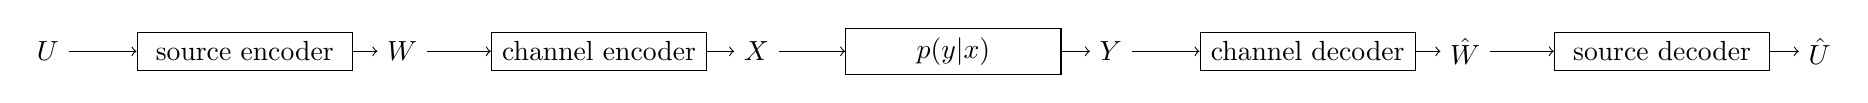
\begin{tikzpicture}[auto, node distance=2cm]

    % Nodes
    \node (U) at (0,0) {$U$};
    \node [draw, rectangle, right of=U, node distance=2.5cm, text width=2.5cm, align=center] (source_encoder) {source encoder};
    \node [right of=source_encoder, node distance=2cm] (W) {$W$};
    \node [draw, rectangle, right of=W, node distance=2.5cm, text width=2.5cm, align=center] (channel_encoder) {channel encoder};
    \node [right of=channel_encoder, node distance=2cm] (X) {$X$};
    \node [draw, rectangle, right of=X, node distance=2.5cm, text width=2.5cm, align=center] (channel) {$p(y|x)$};
    \node [right of=channel, node distance=2cm] (Y) {$Y$};
    \node [draw, rectangle, right of=Y, node distance=2.5cm, text width=2.5cm, align=center] (channel_decoder) {channel decoder};
    \node [right of=channel_decoder, node distance=2cm] (W_hat) {$\hat{W}$};
    \node [draw, rectangle, right of=W_hat, node distance=2.5cm, text width=2.5cm, align=center] (source_decoder) {source decoder};
    \node [right of=source_decoder, node distance=2cm] (U_hat) {$\hat{U}$};
    
    % Arrows
    \draw[->] (U) -- (source_encoder);
    \draw[->] (source_encoder) -- (W);
    \draw[->] (W) -- (channel_encoder);
    \draw[->] (channel_encoder) -- (X);
    \draw[->] (X) -- (channel);
    \draw[->] (channel) -- (Y);
    \draw[->] (Y) -- (channel_decoder);
    \draw[->] (channel_decoder) -- (W_hat);
    \draw[->] (W_hat) -- (source_decoder);
    \draw[->] (source_decoder) -- (U_hat);
\end{tikzpicture}
    \item Choose $R_s$ and $R_c$ such that \[
    H < R_s < R_c < C
    \]

    \item it can be shown that even with complete feedback, reliable communication is impossible if $H>C$
    \item The source code and the channel code can be designed separately without losing asymptotic optimality
    \item The source coding removes redundancy while the channel coding adds redundancy.
 \end{itemize}
\end{document}